% Modelo cinemático continuo de dirección Ackermann (modelo de bicicleta, vista superior).
% Notación de la subsección "Modelo de Dirección de Ackermann" (fundamentos_teoricos.tex).
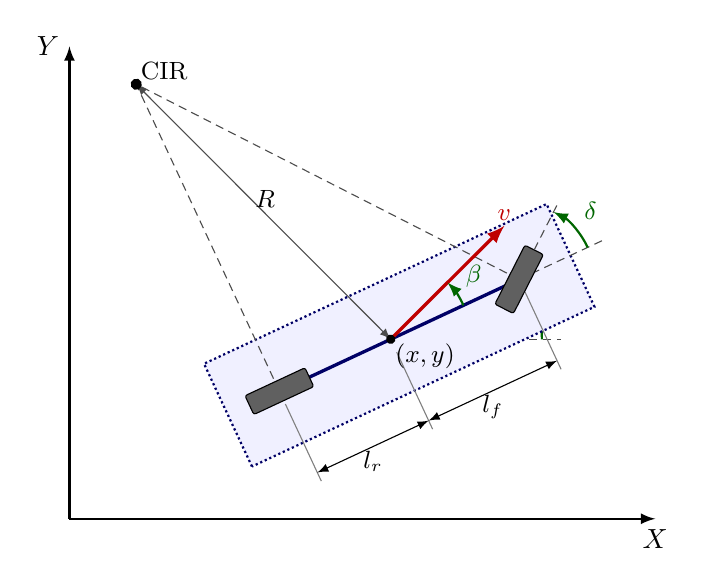
\begin{tikzpicture}[scale=1.2, >=latex,
        cuerpo/.style={fill=blue!12, draw=blue!40!black, thick},
        rueda/.style={fill=gray!75!black, draw=black, rounded corners=0.8pt},
        loca/.style={fill=white, draw=black},
        veloc/.style={->, very thick, red!75!black},
        angulo/.style={->, thick, green!40!black},
        guia/.style={gray!60!black, densely dashed},
        cota/.style={<->, thin},
        etiq/.style={font=\small, inner sep=1.5pt},
        ejes/.style={->, thick}]
\def\psiA{25}      % rumbo psi (grados)
\def\delA{38}      % ángulo de dirección delta (grados)
\def\lr{1.3}       % distancia CM - eje trasero
\def\lf{1.5}       % distancia CM - eje delantero
\pgfmathsetmacro{\LA}{\lr+\lf}
% CIR: corte de las perpendiculares a ambas ruedas
\pgfmathsetmacro{\RyA}{\LA/tan(\delA)}
% Ángulo de deslizamiento beta = atan(lr/(lf+lr) tan delta)
\pgfmathsetmacro{\betA}{atan(\lr/\LA*tan(\delA))}
% Ejes globales
\draw[ejes] (0,0) -- (6.2,0) node[below] {$X$};
\draw[ejes] (0,0) -- (0,5.0) node[left] {$Y$};
% Referencia horizontal para el rumbo
\draw[guia] (3.4,1.9) -- (5.2,1.9);
\draw[angulo] (3.4,1.9) ++(0:1.6) arc (0:\psiA:1.6);
\path (3.4,1.9) ++(10:1.85) node[etiq, text=green!40!black] {$\psi$};
\begin{scope}[shift={(3.4,1.9)}, rotate=\psiA]
    % Contorno del vehículo real
    \draw[cuerpo, densely dotted, fill=blue!6] (-1.9,-0.6) rectangle (2.1,0.6);
    % Perpendiculares a las ruedas hasta el CIR
    \draw[guia] (-\lr,0) -- (-\lr,\RyA);
    \draw[guia] (\lf,0) -- (-\lr,\RyA);
    \draw[cota, gray!60!black] (0,0) -- (-\lr,\RyA)
        node[etiq, pos=0.55, right, text=black] {$R$};
    \fill[black] (-\lr,\RyA) circle (0.06)
        node[etiq, above right] {CIR};
    % Eje longitudinal y su prolongación
    \draw[very thick, blue!40!black] (-\lr,0) -- (\lf,0);
    \draw[guia] (\lf,0) -- (\lf+1.0,0);
    % Rueda trasera (fija) y delantera (orientable)
    \draw[rueda] (-\lr-0.35,-0.11) rectangle (-\lr+0.35,0.11);
    \begin{scope}[shift={(\lf,0)}, rotate=\delA]
        \draw[rueda] (-0.35,-0.11) rectangle (0.35,0.11);
        \draw[guia] (0.35,0) -- (0.9,0);
    \end{scope}
    \draw[angulo] (\lf,0) ++(0:0.8) arc (0:\delA:0.8);
    \path (\lf,0) ++(\delA/2:1.05) node[etiq, text=green!40!black] {$\delta$};
    % Velocidad en el centro de masas y ángulo de deslizamiento
    \draw[veloc] (0,0) -- (\betA:1.7)
        node[etiq, above, text=red!75!black] {$v$};
    \draw[angulo] (0:0.85) arc (0:\betA:0.85);
    \node[etiq, text=green!40!black] at (\betA/2+2:1.1) {$\beta$};
    % Cotas l_r y l_f
    \draw[thin, gray] (-\lr,-0.15) -- (-\lr,-1.05) (0,-0.15) -- (0,-1.05)
        (\lf,-0.15) -- (\lf,-1.05);
    \draw[cota] (-\lr,-0.95) -- (0,-0.95) node[etiq, midway, below] {$l_r$};
    \draw[cota] (0,-0.95) -- (\lf,-0.95) node[etiq, midway, below] {$l_f$};
    % Centro de masas (x, y)
    \fill[black] (0,0) circle (0.05);
\end{scope}
\node[etiq, below right] at (3.4,1.9) {$(x,y)$};
\end{tikzpicture}
